
%% bare_jrnl.tex
%% V1.4a
%% 2014/09/17
%% by Michael Shell
%% see http://www.michaelshell.org/
%% for current contact information.
%%
%% This is a skeleton file demonstrating the use of IEEEtran.cls
%% (requires IEEEtran.cls version 1.8a or later) with an IEEE
%% journal paper.
%%
%% Support sites:
%% http://www.michaelshell.org/tex/ieeetran/
%% http://www.ctan.org/tex-archive/macros/latex/contrib/IEEEtran/
%% and
%% http://www.ieee.org/

%%*************************************************************************
%% Legal Notice:
%% This code is offered as-is without any warranty either expressed or
%% implied; without even the implied warranty of MERCHANTABILITY or
%% FITNESS FOR A PARTICULAR PURPOSE! 
%% User assumes all risk.
%% In no event shall IEEE or any contributor to this code be liable for
%% any damages or losses, including, but not limited to, incidental,
%% consequential, or any other damages, resulting from the use or misuse
%% of any information contained here.
%%
%% All comments are the opinions of their respective authors and are not
%% necessarily endorsed by the IEEE.
%%
%% This work is distributed under the LaTeX Project Public License (LPPL)
%% ( http://www.latex-project.org/ ) version 1.3, and may be freely used,
%% distributed and modified. A copy of the LPPL, version 1.3, is included
%% in the base LaTeX documentation of all distributions of LaTeX released
%% 2003/12/01 or later.
%% Retain all contribution notices and credits.
%% ** Modified files should be clearly indicated as such, including  **
%% ** renaming them and changing author support contact information. **
%%
%% File list of work: IEEEtran.cls, IEEEtran_HOWTO.pdf, bare_adv.tex,
%%                    bare_conf.tex, bare_jrnl.tex, bare_conf_compsoc.tex,
%%                    bare_jrnl_compsoc.tex, bare_jrnl_transmag.tex
%%*************************************************************************


% *** Authors should verify (and, if needed, correct) their LaTeX system  ***
% *** with the testflow diagnostic prior to trusting their LaTeX platform ***
% *** with production work. IEEE's font choices and paper sizes can       ***
% *** trigger bugs that do not appear when using other class files.       ***                          ***
% The testflow support page is at:
% http://www.michaelshell.org/tex/testflow/



\documentclass[journal]{IEEEtran}
%
% If IEEEtran.cls has not been installed into the LaTeX system files,
% manually specify the path to it like:
% \documentclass[journal]{../sty/IEEEtran}





% Some very useful LaTeX packages include:
% (uncomment the ones you want to load)


% *** MISC UTILITY PACKAGES ***
%
%\usepackage{ifpdf}
% Heiko Oberdiek's ifpdf.sty is very useful if you need conditional
% compilation based on whether the output is pdf or dvi.
% usage:
% \ifpdf
%   % pdf code
% \else
%   % dvi code
% \fi
% The latest version of ifpdf.sty can be obtained from:
% http://www.ctan.org/tex-archive/macros/latex/contrib/oberdiek/
% Also, note that IEEEtran.cls V1.7 and later provides a builtin
% \ifCLASSINFOpdf conditional that works the same way.
% When switching from latex to pdflatex and vice-versa, the compiler may
% have to be run twice to clear warning/error messages.






% *** CITATION PACKAGES ***
%
%\usepackage{cite}
% cite.sty was written by Donald Arseneau
% V1.6 and later of IEEEtran pre-defines the format of the cite.sty package
% \cite{} output to follow that of IEEE. Loading the cite package will
% result in citation numbers being automatically sorted and properly
% "compressed/ranged". e.g., [1], [9], [2], [7], [5], [6] without using
% cite.sty will become [1], [2], [5]--[7], [9] using cite.sty. cite.sty's
% \cite will automatically add leading space, if needed. Use cite.sty's
% noadjust option (cite.sty V3.8 and later) if you want to turn this off
% such as if a citation ever needs to be enclosed in parenthesis.
% cite.sty is already installed on most LaTeX systems. Be sure and use
% version 5.0 (2009-03-20) and later if using hyperref.sty.
% The latest version can be obtained at:
% http://www.ctan.org/tex-archive/macros/latex/contrib/cite/
% The documentation is contained in the cite.sty file itself.






% *** GRAPHICS RELATED PACKAGES ***
%
\ifCLASSINFOpdf
  \usepackage[pdftex]{graphicx}
  % declare the path(s) where your graphic files are
  % \graphicspath{{../pdf/}{../jpeg/}}
  % and their extensions so you won't have to specify these with
  % every instance of \includegraphics
  % \DeclareGraphicsExtensions{.pdf,.jpeg,.png}
\else
  % or other class option (dvipsone, dvipdf, if not using dvips). graphicx
  % will default to the driver specified in the system graphics.cfg if no
  % driver is specified.
  \usepackage[dvips]{graphicx}
  % declare the path(s) where your graphic files are
  % \graphicspath{{../eps/}}
  % and their extensions so you won't have to specify these with
  % every instance of \includegraphics
  % \DeclareGraphicsExtensions{.eps}
\fi
% graphicx was written by David Carlisle and Sebastian Rahtz. It is
% required if you want graphics, photos, etc. graphicx.sty is already
% installed on most LaTeX systems. The latest version and documentation
% can be obtained at: 
% http://www.ctan.org/tex-archive/macros/latex/required/graphics/
% Another good source of documentation is "Using Imported Graphics in
% LaTeX2e" by Keith Reckdahl which can be found at:
% http://www.ctan.org/tex-archive/info/epslatex/
%
% latex, and pdflatex in dvi mode, support graphics in encapsulated
% postscript (.eps) format. pdflatex in pdf mode supports graphics
% in .pdf, .jpeg, .png and .mps (metapost) formats. Users should ensure
% that all non-photo figures use a vector format (.eps, .pdf, .mps) and
% not a bitmapped formats (.jpeg, .png). IEEE frowns on bitmapped formats
% which can result in "jaggedy"/blurry rendering of lines and letters as
% well as large increases in file sizes.
%
% You can find documentation about the pdfTeX application at:
% http://www.tug.org/applications/pdftex





% *** MATH PACKAGES ***
%
%\usepackage[cmex10]{amsmath}
% A popular package from the American Mathematical Society that provides
% many useful and powerful commands for dealing with mathematics. If using
% it, be sure to load this package with the cmex10 option to ensure that
% only type 1 fonts will utilized at all point sizes. Without this option,
% it is possible that some math symbols, particularly those within
% footnotes, will be rendered in bitmap form which will result in a
% document that can not be IEEE Xplore compliant!
%
% Also, note that the amsmath package sets \interdisplaylinepenalty to 10000
% thus preventing page breaks from occurring within multiline equations. Use:
%\interdisplaylinepenalty=2500
% after loading amsmath to restore such page breaks as IEEEtran.cls normally
% does. amsmath.sty is already installed on most LaTeX systems. The latest
% version and documentation can be obtained at:
% http://www.ctan.org/tex-archive/macros/latex/required/amslatex/math/





% *** SPECIALIZED LIST PACKAGES ***
%
%\usepackage{algorithmic}
% algorithmic.sty was written by Peter Williams and Rogerio Brito.
% This package provides an algorithmic environment fo describing algorithms.
% You can use the algorithmic environment in-text or within a figure
% environment to provide for a floating algorithm. Do NOT use the algorithm
% floating environment provided by algorithm.sty (by the same authors) or
% algorithm2e.sty (by Christophe Fiorio) as IEEE does not use dedicated
% algorithm float types and packages that provide these will not provide
% correct IEEE style captions. The latest version and documentation of
% algorithmic.sty can be obtained at:
% http://www.ctan.org/tex-archive/macros/latex/contrib/algorithms/
% There is also a support site at:
% http://algorithms.berlios.de/index.html
% Also of interest may be the (relatively newer and more customizable)
% algorithmicx.sty package by Szasz Janos:
% http://www.ctan.org/tex-archive/macros/latex/contrib/algorithmicx/




% *** ALIGNMENT PACKAGES ***
%
%\usepackage{array}
% Frank Mittelbach's and David Carlisle's array.sty patches and improves
% the standard LaTeX2e array and tabular environments to provide better
% appearance and additional user controls. As the default LaTeX2e table
% generation code is lacking to the point of almost being broken with
% respect to the quality of the end results, all users are strongly
% advised to use an enhanced (at the very least that provided by array.sty)
% set of table tools. array.sty is already installed on most systems. The
% latest version and documentation can be obtained at:
% http://www.ctan.org/tex-archive/macros/latex/required/tools/


% IEEEtran contains the IEEEeqnarray family of commands that can be used to
% generate multiline equations as well as matrices, tables, etc., of high
% quality.




% *** SUBFIGURE PACKAGES ***
%\ifCLASSOPTIONcompsoc
%  \usepackage[caption=false,font=normalsize,labelfont=sf,textfont=sf]{subfig}
%\else
%  \usepackage[caption=false,font=footnotesize]{subfig}
%\fi
% subfig.sty, written by Steven Douglas Cochran, is the modern replacement
% for subfigure.sty, the latter of which is no longer maintained and is
% incompatible with some LaTeX packages including fixltx2e. However,
% subfig.sty requires and automatically loads Axel Sommerfeldt's caption.sty
% which will override IEEEtran.cls' handling of captions and this will result
% in non-IEEE style figure/table captions. To prevent this problem, be sure
% and invoke subfig.sty's "caption=false" package option (available since
% subfig.sty version 1.3, 2005/06/28) as this is will preserve IEEEtran.cls
% handling of captions.
% Note that the Computer Society format requires a larger sans serif font
% than the serif footnote size font used in traditional IEEE formatting
% and thus the need to invoke different subfig.sty package options depending
% on whether compsoc mode has been enabled.
%
% The latest version and documentation of subfig.sty can be obtained at:
% http://www.ctan.org/tex-archive/macros/latex/contrib/subfig/




% *** FLOAT PACKAGES ***
%
%\usepackage{fixltx2e}
% fixltx2e, the successor to the earlier fix2col.sty, was written by
% Frank Mittelbach and David Carlisle. This package corrects a few problems
% in the LaTeX2e kernel, the most notable of which is that in current
% LaTeX2e releases, the ordering of single and double column floats is not
% guaranteed to be preserved. Thus, an unpatched LaTeX2e can allow a
% single column figure to be placed prior to an earlier double column
% figure. The latest version and documentation can be found at:
% http://www.ctan.org/tex-archive/macros/latex/base/


%\usepackage{stfloats}
% stfloats.sty was written by Sigitas Tolusis. This package gives LaTeX2e
% the ability to do double column floats at the bottom of the page as well
% as the top. (e.g., "\begin{figure*}[!b]" is not normally possible in
% LaTeX2e). It also provides a command:
%\fnbelowfloat
% to enable the placement of footnotes below bottom floats (the standard
% LaTeX2e kernel puts them above bottom floats). This is an invasive package
% which rewrites many portions of the LaTeX2e float routines. It may not work
% with other packages that modify the LaTeX2e float routines. The latest
% version and documentation can be obtained at:
% http://www.ctan.org/tex-archive/macros/latex/contrib/sttools/
% Do not use the stfloats baselinefloat ability as IEEE does not allow
% \baselineskip to stretch. Authors submitting work to the IEEE should note
% that IEEE rarely uses double column equations and that authors should try
% to avoid such use. Do not be tempted to use the cuted.sty or midfloat.sty
% packages (also by Sigitas Tolusis) as IEEE does not format its papers in
% such ways.
% Do not attempt to use stfloats with fixltx2e as they are incompatible.
% Instead, use Morten Hogholm'a dblfloatfix which combines the features
% of both fixltx2e and stfloats:
%
% \usepackage{dblfloatfix}
% The latest version can be found at:
% http://www.ctan.org/tex-archive/macros/latex/contrib/dblfloatfix/




%\ifCLASSOPTIONcaptionsoff
%  \usepackage[nomarkers]{endfloat}
% \let\MYoriglatexcaption\caption
% \renewcommand{\caption}[2][\relax]{\MYoriglatexcaption[#2]{#2}}
%\fi
% endfloat.sty was written by James Darrell McCauley, Jeff Goldberg and 
% Axel Sommerfeldt. This package may be useful when used in conjunction with 
% IEEEtran.cls'  captionsoff option. Some IEEE journals/societies require that
% submissions have lists of figures/tables at the end of the paper and that
% figures/tables without any captions are placed on a page by themselves at
% the end of the document. If needed, the draftcls IEEEtran class option or
% \CLASSINPUTbaselinestretch interface can be used to increase the line
% spacing as well. Be sure and use the nomarkers option of endfloat to
% prevent endfloat from "marking" where the figures would have been placed
% in the text. The two hack lines of code above are a slight modification of
% that suggested by in the endfloat docs (section 8.4.1) to ensure that
% the full captions always appear in the list of figures/tables - even if
% the user used the short optional argument of \caption[]{}.
% IEEE papers do not typically make use of \caption[]'s optional argument,
% so this should not be an issue. A similar trick can be used to disable
% captions of packages such as subfig.sty that lack options to turn off
% the subcaptions:
% For subfig.sty:
% \let\MYorigsubfloat\subfloat
% \renewcommand{\subfloat}[2][\relax]{\MYorigsubfloat[]{#2}}
% However, the above trick will not work if both optional arguments of
% the \subfloat command are used. Furthermore, there needs to be a
% description of each subfigure *somewhere* and endfloat does not add
% subfigure captions to its list of figures. Thus, the best approach is to
% avoid the use of subfigure captions (many IEEE journals avoid them anyway)
% and instead reference/explain all the subfigures within the main caption.
% The latest version of endfloat.sty and its documentation can obtained at:
% http://www.ctan.org/tex-archive/macros/latex/contrib/endfloat/
%
% The IEEEtran \ifCLASSOPTIONcaptionsoff conditional can also be used
% later in the document, say, to conditionally put the References on a 
% page by themselves.




% *** PDF, URL AND HYPERLINK PACKAGES ***
%
\usepackage{url}
% url.sty was written by Donald Arseneau. It provides better support for
% handling and breaking URLs. url.sty is already installed on most LaTeX
% systems. The latest version and documentation can be obtained at:
% http://www.ctan.org/tex-archive/macros/latex/contrib/url/
% Basically, \url{my_url_here}.




% *** Do not adjust lengths that control margins, column widths, etc. ***
% *** Do not use packages that alter fonts (such as pslatex).         ***
% There should be no need to do such things with IEEEtran.cls V1.6 and later.
% (Unless specifically asked to do so by the journal or conference you plan
% to submit to, of course. )


% correct bad hyphenation here
\hyphenation{op-tical net-works semi-conduc-tor}


%RETIRAR DA VERSÃO EM INGLÊS
%\usepackage[brazil]{babel}
\usepackage[utf8]{inputenc}		


\begin{document}
%
% paper title
% Titles are generally capitalized except for words such as a, an, and, as,
% at, but, by, for, in, nor, of, on, or, the, to and up, which are usually
% not capitalized unless they are the first or last word of the title.
% Linebreaks \\ can be used within to get better formatting as desired.
% Do not put math or special symbols in the title.
\title{Um Software coma Serviço para Análise de Marcha}
%
%
% author names and IEEE memberships
% note positions of commas and nonbreaking spaces ( ~ ) LaTeX will not break
% a structure at a ~ so this keeps an author's name from being broken across
% two lines.
% use \thanks{} to gain access to the first footnote area
% a separate \thanks must be used for each paragraph as LaTeX2e's \thanks
% was not built to handle multiple paragraphs
%

\author{Roberto Aguiar Lima,
	Vera Regina Da Silva Marães,
        and Lourdes Mattos Brasil 
\thanks{R. A. Lima e L. M. Brasil são da FGA/UnB}% <-this % stops a space
\thanks{V. R. S. Marães é da FCE/UnB}}% <-this % stops a space

% note the % following the last \IEEEmembership and also \thanks - 
% these prevent an unwanted space from occurring between the last author name
% and the end of the author line. i.e., if you had this:
% 
% \author{....lastname \thanks{...} \thanks{...} }
%                     ^------------^------------^----Do not want these spaces!
%
% a space would be appended to the last name and could cause every name on that
% line to be shifted left slightly. This is one of those "LaTeX things". For
% instance, "\textbf{A} \textbf{B}" will typeset as "A B" not "AB". To get
% "AB" then you have to do: "\textbf{A}\textbf{B}"
% \thanks is no different in this regard, so shield the last } of each \thanks
% that ends a line with a % and do not let a space in before the next \thanks.
% Spaces after \IEEEmembership other than the last one are OK (and needed) as
% you are supposed to have spaces between the names. For what it is worth,
% this is a minor point as most people would not even notice if the said evil
% space somehow managed to creep in.



% The paper headers
\markboth{Journal of \LaTeX\ Class Files,~Vol.~13, No.~9, September~2014}%
{Shell \MakeLowercase{\textit{et al.}}: Bare Demo of IEEEtran.cls for Journals}
% The only time the second header will appear is for the odd numbered pages
% after the title page when using the twoside option.
% 
% *** Note that you probably will NOT want to include the author's ***
% *** name in the headers of peer review papers.                   ***
% You can use \ifCLASSOPTIONpeerreview for conditional compilation here if
% you desire.




% If you want to put a publisher's ID mark on the page you can do it like
% this:
%\IEEEpubid{0000--0000/00\$00.00~\copyright~2014 IEEE}
% Remember, if you use this you must call \IEEEpubidadjcol in the second
% column for its text to clear the IEEEpubid mark.



% use for special paper notices
%\IEEEspecialpapernotice{(Invited Paper)}




% make the title area
\maketitle

% As a general rule, do not put math, special symbols or citations
% in the abstract or keywords.
\begin{abstract}
	Este trabalho descreve o desenvolvimento da primeira versão
	de um software como serviço para análise e simulação de marcha
	humana. 
	A principal vantagem deste enfoque é a disponibilização via web
	do software. Depois de implantado num servidor central, os usuários
	poderão acessar o software através de um browser recente que suporte HTML 5. 
	O objetivo do software é minimizar a necessidade de 
	pesquisadores da área de escrever código em suas pesquisas.
	O software permite importar dados gerados de marcadores de superfície a partir de um
	sistema de captura de movimentos, plotar a progressão espacial destes marcadores,
	os ângulos, velocidades angulares e acelerações angulares dos marcadores.
	Além disso é possivel visualizar os marcadores numa animação em 3D.
	O código fonte está disponível como software livre e frequentemente recebe novas
	funcionalidades, sendo que uma nova comunidade está sendo criada em torno do software.
\end{abstract}

% Note that keywords are not normally used for peerreview papers.
\begin{IEEEkeywords}
	Análise de marcha, software como serviço.
\end{IEEEkeywords}

% For peer review papers, you can put extra information on the cover
% page as needed:
% \ifCLASSOPTIONpeerreview
% \begin{center} \bfseries EDICS Category: 3-BBND \end{center}
% \fi
%
% For peerreview papers, this IEEEtran command inserts a page break and
% creates the second title. It will be ignored for other modes.
\IEEEpeerreviewmaketitle



\section{Introduction}
% The very first letter is a 2 line initial drop letter followed
% by the rest of the first word in caps.
% 
% form to use if the first word consists of a single letter:
% \IEEEPARstart{A}{demo} file is ....
% 
% form to use if you need the single drop letter followed by
% normal text (unknown if ever used by IEEE):
% \IEEEPARstart{A}{}demo file is ....
% 
% Some journals put the first two words in caps:
% \IEEEPARstart{T}{his demo} file is ....
% 
% Here we have the typical use of a "T" for an initial drop letter
% and "HIS" in caps to complete the first word.
\IEEEPARstart{C}{om} o advento da internet foi possível criar serviços 
que podem ser implementados e implantados num servidor central e 
disponibilados para qualquer parte do mundo. 
Além disso, os browsers webs modernos se tornaram uma verdadeira plataforma,
permitindo a criação de interfaces de usuário ricas, inclusive com apresentação 
de gráficos e animações em 3D. 

Estas duas tecnologias, servidores e browsers web, podem ser 
usadas como base para o que se conhece como software como serviço. 
Em \cite{Fox2012} são citadas vária vantagens desta abordagem, 
destacando-se entre elas a fácil disponibilização do software,
por exemplo, o usuário do software não precisa instalar uma 
versão do software em seu computador, basta acessá-lo pelo
browser web que o sistema estará disponível.

Segundo \cite{Baker2007}, apesar dos avanços ocorridos na análise de marcha 
até meados do meio do século
vinte, foi só após o advento dos computadores modernos 
que a análise de marcha clínica
tornou-se amplamente disponível. Pacotes do software para análise de marcha foram
implementados \cite{Moraes2003}.
Mas até agora no século 21, nenhum fornecedor de software comprometeu-se
a
entregar um sistema de análise de máquina disponibilizado como serviço na web,
em outras palavras, profissionais de saúde ou pesquisadores de análisde de marcha
que querem usar um software para isto, têm que utilizar software instalados
numa máquina com arquitetura específica e sistema operacional específico. 
Eles ficam responsáveis por backups dos dados,
ao surgirem novas funcionalidades no software, os mesmos têm que instalá-lo
novamente, se eles quiserem compartilhar dados terão que copiá-los e enviá-los
a seu destinatário. 
Todos esses problemas são eliminados quando se utiliza Software como Serviço.
Além disto técnicas de análise de marcha são bem documentadas hoje em dia
\cite{Perry2010} \cite{Skinner2007} \cite{Ferreira2009}, o que facilita a escolha de características a serem adotados
para um software.
Com isto em mente, o presente trabalho descreve a implementação
de um software como serviço para análise de marcha, que foi
inicialmente concebido por \cite{Lima2015}. 
O software implementado é capaz de recuperar dados gerados por um sistema de
captura de imagens, no caso dados de  marcadores de superfície, 
nomear marcadores,
gerar gráficos de progreção espacial dos marcadores, 
definir ângulos usando os marcadores, plotar gráficos dos ângulos, 
velocidades angulares e acelerações angulares, além de exibir uma animação
interativa em 3D dos marcadores.

% You must have at least 2 lines in the paragraph with the drop letter
% (should never be an issue)

\section{Metodologia}
Dois ambientes de pesquisa foram utilizados, um foi o Laboratório de 
Performance Human (LPH) na Faculdade Ceilândia (FCE) 
da Universidade de Brasília (UnB), e o Laboratório de Informática em Saúde
(LIS) na Faculdade Gama (FGA) da UnB.
No LPH foram coletados os dados e no LIS foi desenvolvido o software.

O projeto no qual ocorreu a coleta foi aprovado pelo Comitê de Ética
da Faculdade de Saúde da UnB, processo N11911/12.

\subsection{Coleta de Dados}
Os dados coletados foram captados através de câmeras Oqus MRI da
Qualisys usando-se o software QTM do mesmo fabricante. 
Os dados são referentes a marcadores de superfície
dispostos ao longo do corpo do paciente.
O processo de coleta é descrito na Fig. \ref{coleta_dados}.
Para este trabalho um paciente saudável do sexo masculino com idade entre 20 e 30 anos
foi selecionado.
Também é necessario definir quais os pontos no corpo do paciente devem
receber marcadores de superfıcie, neste caso os pontos de interesse foram o trocanter esquerdo, joelho esquerdo e tíbia esquerda. 
O proximo passo se refere a coleta dos dados em si. 
O paciente deve repetir um ciclo de marcha confortavel de aproximadamente 5 segundos,
por 5 vezes na frente das câmeras.
Os dados devem ser convertidos para formato adequado à linguagem
MATLAB. Esta opção está disponível no QTM. 
\begin{figure}[!t]
	\centering
	{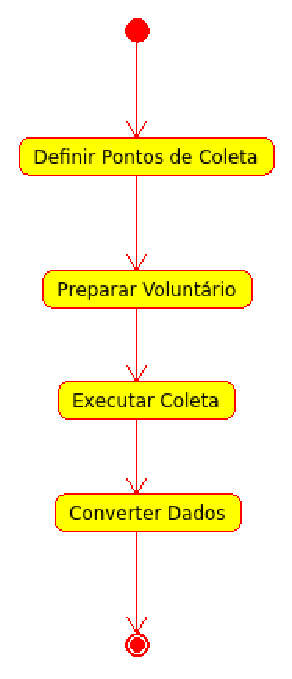
\includegraphics[width=4cm]{coleta_dados}}
	\caption{Processo de coleta de dados.}
	\label{coleta_dados}
\end{figure}

\subsection{Processo de desenvolvimento}
O processo de desenvolvimento foi inspirado no scrum \cite{Schwaber2001}.
O scrum é um porcesso de desenvolvimento ágil \cite{Beck2001}, que tem como
principais características ser iterativo e incremental. Estas características
são essenciais para lidar com a natureza volátil dos requisitos de software.

O arcabouço do processo pode ser visto na Fig. \ref{dev_proc}. O processo
consiste de iterações, chamadas de sprint, que duram em média duas
semanas. Um backlog de produto é administrado por um product owner. 
Este backlog fica sempre em aberto, recebendo adições na forma de
histórias do usuário \cite{cohn2004}. Antes de cada iteração uma reunião
com a equipe é feita. Esta reunião é dividida em duas fases. Na primeira
fase são apresentados os resultados da última iteração. Na segunda fase
histórias do usuário contidas no backlog do produto são selecionadas.
Estas histórias compõe o backlog do sprint, que são as funcionalidades a serem implementadas
durante o sprint. Ao final do sprint
um incremento é produzido. O incremento consiste num pedaço de software
funcional pronto para ser implantado.

\begin{figure}[!t]
	\centering
	{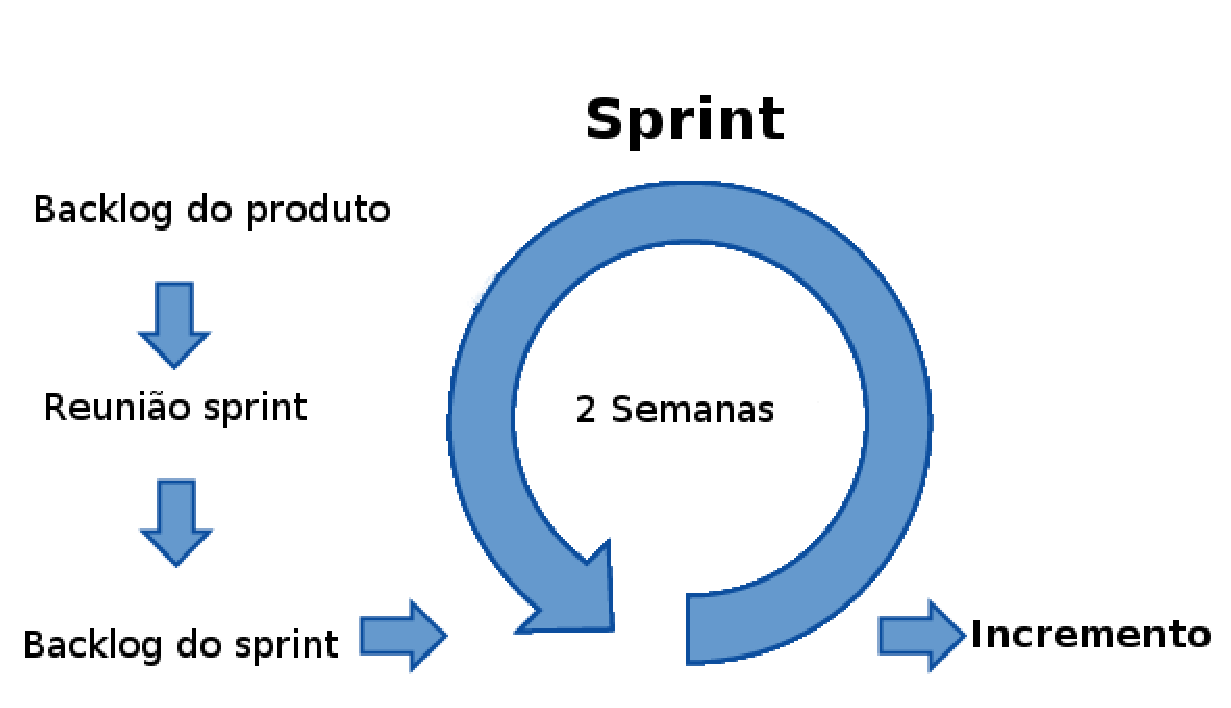
\includegraphics[width=8cm]{scrum_projeto}}
	\caption{Processo de desenvolvimento.}
	\label{dev_proc}
\end{figure}


\subsection{Arquitetura da Aplicação}
A Fig. \ref{camadas} mostra uma visão de alto nível da
arquitetura do software. A camada web é responsável pela interação com o usuário. 
A camada Web API  é responsável pela lógica de negócio. 
A camada de base de documentos é responsável pela
persistência dos dados da aplicação.
\begin{figure}[!t]
	\centering
	{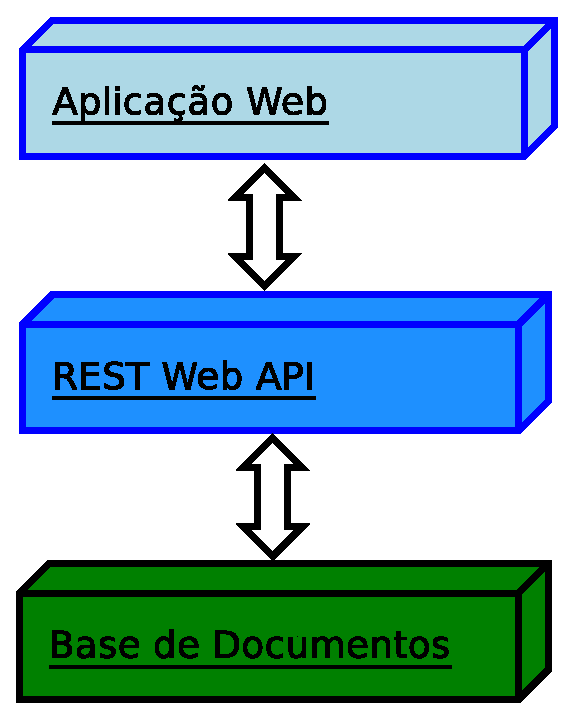
\includegraphics[width=4cm]{camadas}}
	\caption{Visão de alto nível da arquitetura.}
	\label{camadas}
\end{figure}

\subsubsection{Camada Web}
Esta camada foi projetada para rodar em browsers que suportam HTML 5. Ela é 
desenvolvida usando-se Javascript, CSS e HTML. Além disso, adotou-se o framework de
desenvolvimento web AngularJS. Esta tecnologia foi descrita em \cite{Branas2014}.
Uma das vantagens de se usar o AngularJS é a possibilidade de se criar diretivas.
Diretivas são componentes que podem ser embutidas num template HTML.
Neste projeto também foi utilizada a biblioteca de diretivas Angular-Material.
Esta biblioteca é baseada na especificação Material Design criada pela empresa Google. 
A especificação discorre sobre padrões de designe gráfico e interação com usuário e é baseada 
no princípio da metáfora de materiais. 
Segundo \cite{Google2015a}, esta metáfora é uma teoria unificada de um espaço racionalizado
e sistemas de movimento. A intenção da escolha desta biblioteca foi a de criar
uma experiência de usuário aceitável para profissionais da área de sáude.

Para executar animações gráficas em 3D, foi utilizada a biblioteca ThreeJS, descrita em \cite{Dirksen2015}.
Esta é uma biblioteca de alto nível que se aproveita do padrão WebGL, implementado
nos broswers webs recentes. O padrão WebGL, ver \cite{Matsuda2013} usa nativamente a GPU do computardor, 
permitindo assim criar aplicações que necessitam boa performance para gerar
gráficos. 

A Fig. \ref{camada_web} mostra a interação entre os principais componentes da camada web.
O usuário ao interagir com a aplicação, através de seu browser, dispara algum evento, 
por exemplo, um clique num botão. O framework AngularJS detecta o evento e o repassa
para um controlador desenvolvido especiamente para a aplicação. Caso seja necessária 
a execução de alguma lógica de negócio e dados da aplicação, o controlador faz uma
requisição para uma Facade, também desenvolvida para a aplicação. Esta Facade é responsável
por encapsular a requisição transformado-a numa requisição HTTP para o backend, ou seja, 
o servidor da aplicação na internet. Despois da resposta, que vem no formato JSON, ser
enviada pelo backend e recebida pela Facade, esta a encaminha para o Controlador que
fica responsável por executar a lógica necessária para os dados serem apresentados ao 
usuário.

\begin{figure*}[tb]
	\centering
	{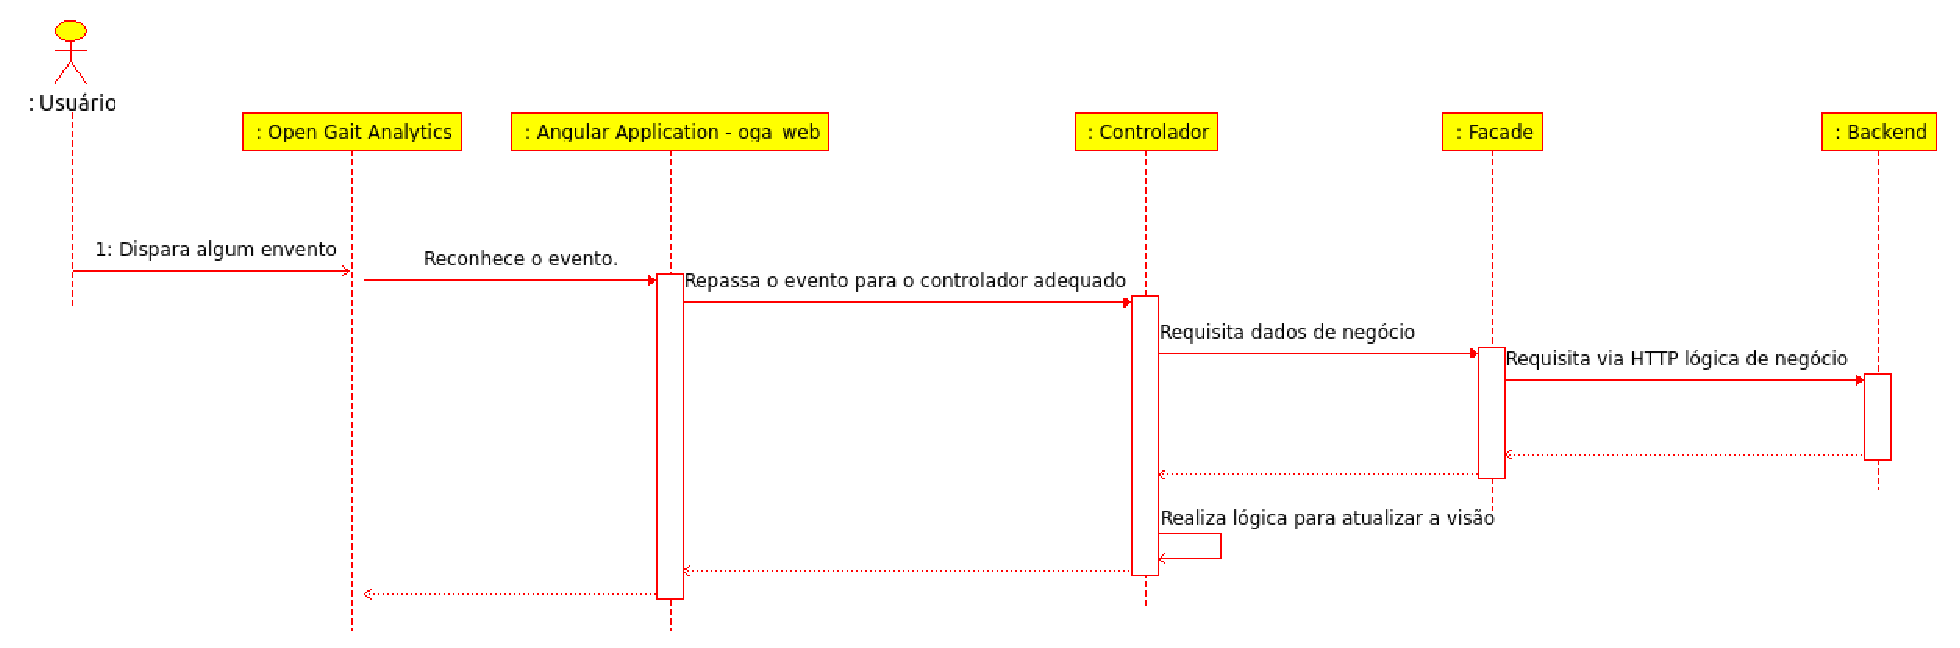
\includegraphics[width=\textwidth]{camada_web}}
	\caption{Interação dos componentes da camada Web.  O usuário, usando o seu browser web, interage com a aplicação, clicando num botão por exemplo, o framework AngularJS reconhece o evento e dispara o procedimento corrento para tratá-lo, que está dentro de uma classe controladora. Caso seja necessário recuperar algum dado no backend, o controlador delega esta tarefa para uma classe Facade.}
	\label{camada_web}
\end{figure*}

\subsubsection{Camada REST Web API}

Esta camada é responsável pela execução da lógica de negócio, como por exemplo,
fazer cálculos de ângulos e extrair dados do arquivo em formato MATLAB proveniente do QTM.
Esta camada foi implementada usando-se o estilo arquitetural Representational Estate Transfer (REST),
descrito por \cite{Grinberg2014}. A maior vantagem desta tecnologia é o alto desacoplamento com a
camada web. Para implementar este estilo foi escolhido o framework Flask \cite{Maia2015}. Esta é 
uma biblioteca escrita em Python,  que segundo \cite{Maia2015} é conhecida por sua filosofia minimalista,
permitindo-se criar um projeto simples no início, mas que permite evolução para modelos
mais complexos conforme a necessidade do momento.

A Fig. \ref{camada_api} mostra a interação entre alguns componentes da camada REST Web API.
Depois do browser do usuário encaminhar a requisição HTTP para o servidore web, este o 
encaminha para a aplicação escrita em Python com o framework Flask, o framework roteia
a requisição para uma função escrita em Python, esta pode acessar bibliotecas disponíveis
para a aplicação ou fazer uma consulta ao banco de documentos através da biblioteca PyMongo.
A lógica de negócio pode ser implementada dentro desta função, ou caso seja muito complexa,
numa biblioteca escrita especiamente para a funcinalidade.
Depois de processado o resultado é convertido para o formato JSON e retornado para o browser
do usuário.

\begin{figure*}[tb]
	\centering
	{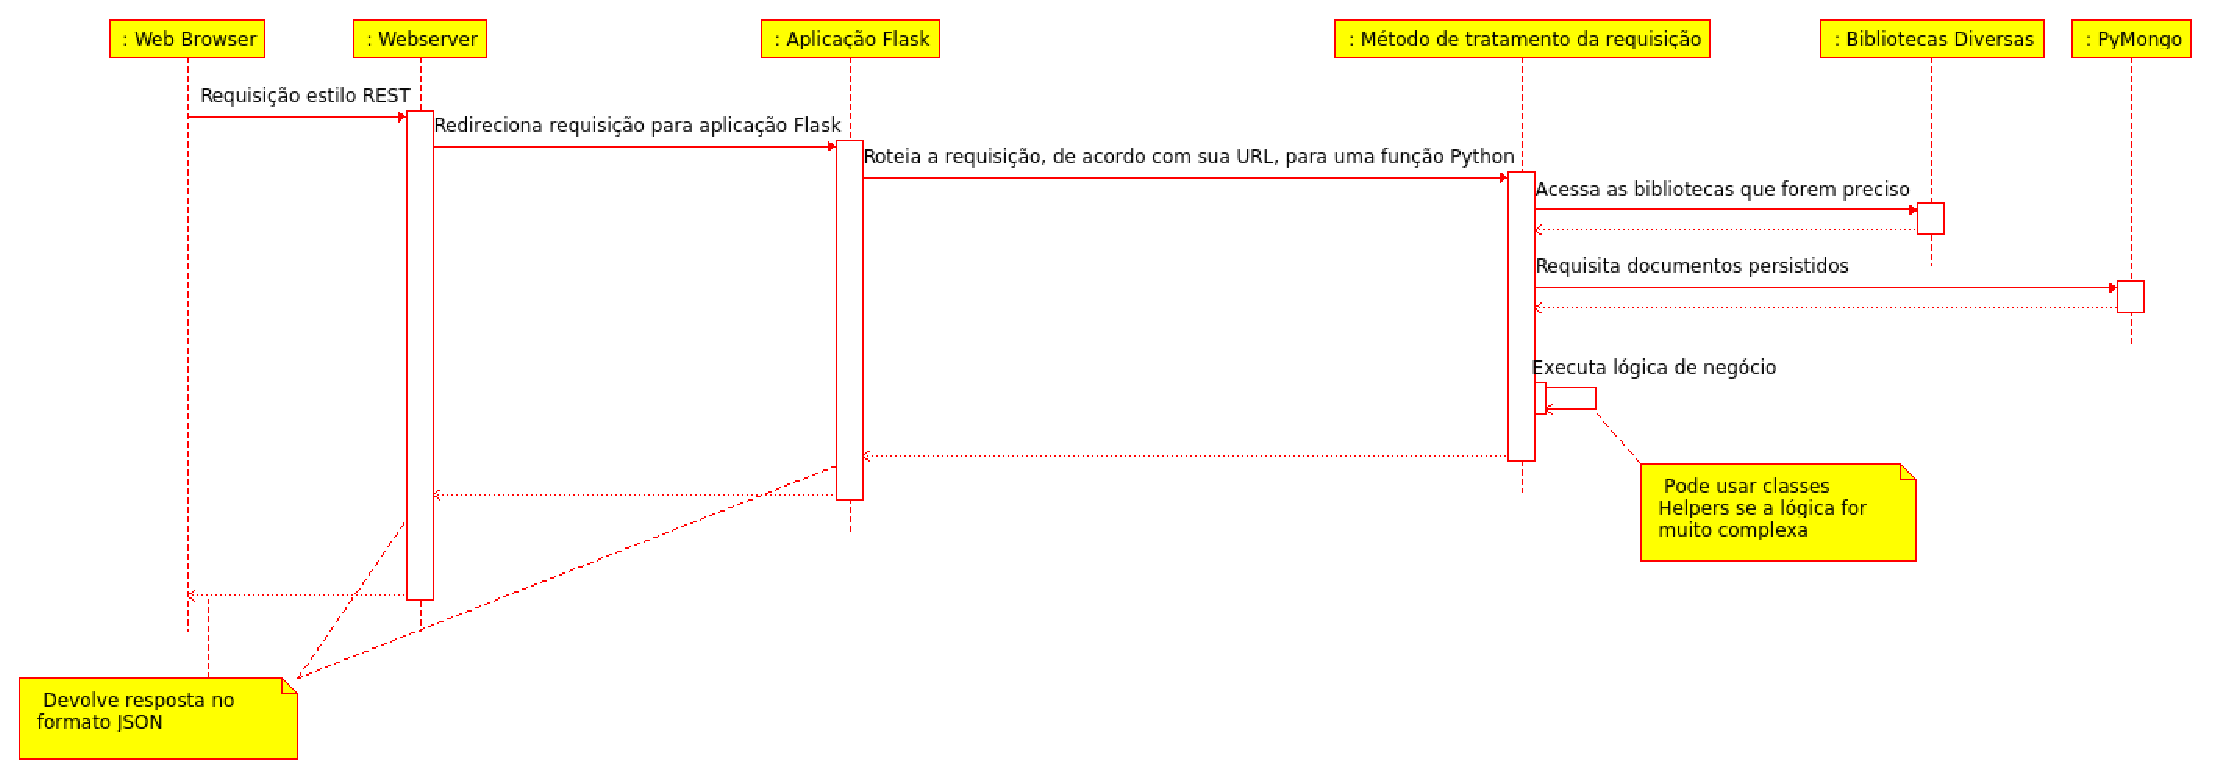
\includegraphics[width=\textwidth]{camada_api}}
	\caption{Interação dos componentes da camada REST Web API. Quando a aplicação web necessita de dados, ela faz uma requisição HTTP a camada REST Web API. Esta requisição é recebida pelo servidor web que a redireciona para a aplicação Flask. A aplicação Flask identifica a requisição e a encaminha para uma função Python apropriada para ser processada. Esta função tem acesso a diversas bibliotecas para ajudar no processamento, como NumPy, Matplotlib, bibliotecas específicas da aplicação entre outras.  Se algum dado persistido for necessário, também pode-se utilizar a biblioteca PyMongo para buscá-los na base de documentos. Finalmente uma resposta HTTP é criada. O conteúdo desta resposta é um objeto no formato JSON que será consumido pela camada web.}
	\label{camada_api}
\end{figure*}

\subsubsection{Camada de Base de Documentos}

A camada de base de documentos é responsável pela persistência dos dados da aplicação.
Esta camada basicamente é formada por uma base implementada usando-se a tecnologia
MongoDB. Uma introdução ao MongoDB é feita em \cite{Plugge2014}.
A escolha desta tecnologia, em detrimento a um banco de dados relacional que é mais comum,
foi devido a natureza multidimensional dos dados, que é mais facilmente modelada num
banco de documento, e também por causa das facilidades relativas a escalabilidade do 
MongoDB.
A Fig. \ref{mongo_oga} mostra a base de dados oga, que possui duas coleções de dados 
patients e positionals\_data.

\begin{figure}[!t]
	\centering
	{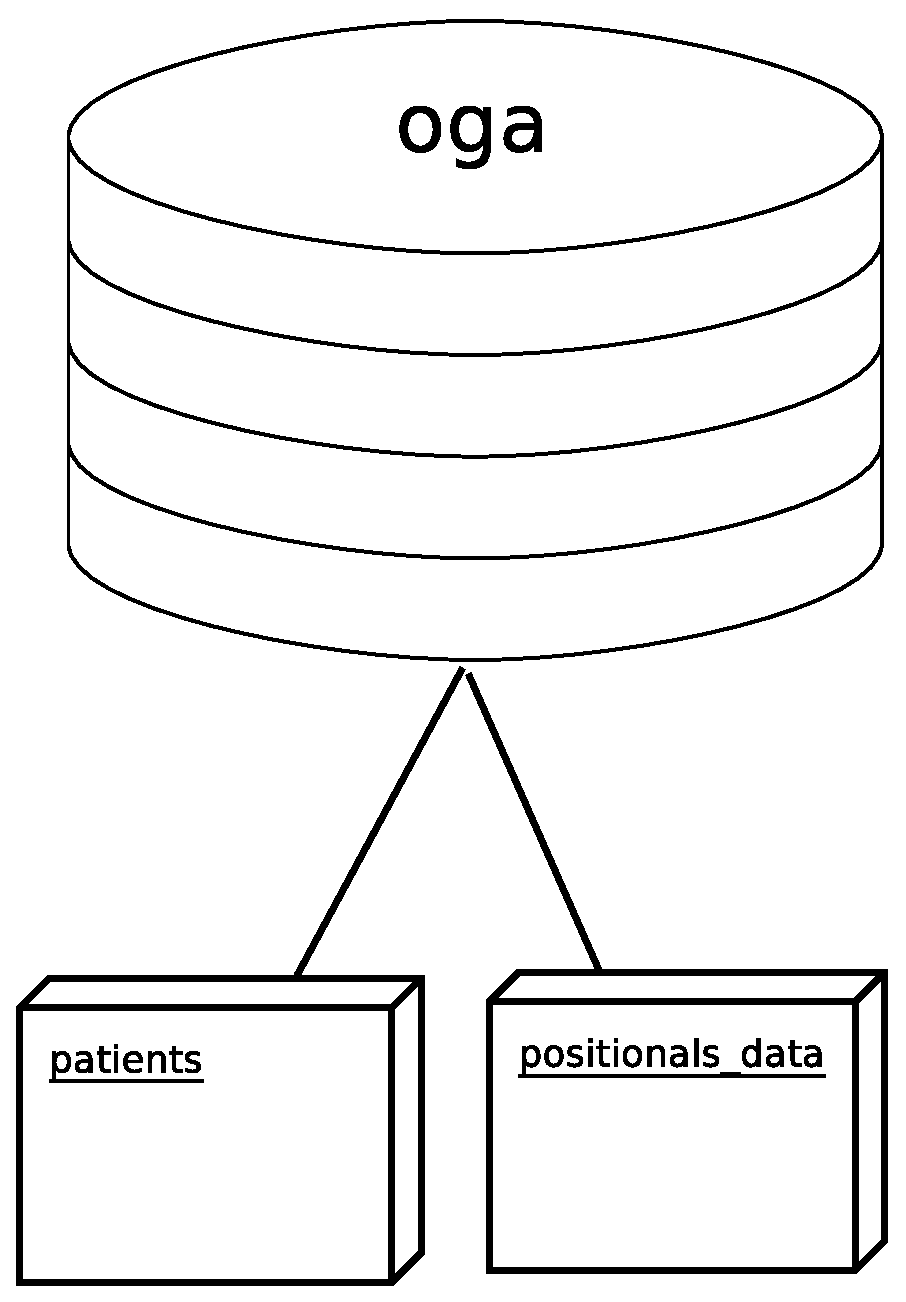
\includegraphics[width=4cm]{mongo_oga}}
	\caption{Base de documentos da aplicação. }
	\label{mongo_oga}
\end{figure}

\section{Resultados}
O software desenvolvido permite o cadastro de pacientes e de amostras de dados espaciais
coletadas pelo software QTM. 
Depois de se cadastrar o paciente, o usuário deve incluir uma nova amostra de dados.
Para isso ele deve importar o arquivo com a amostra para o sistema. Após o processo de 
importação a tela descrita na Fig. \ref{qtm_data} é mostrada.

\begin{figure*}[tb]
	\centering
	{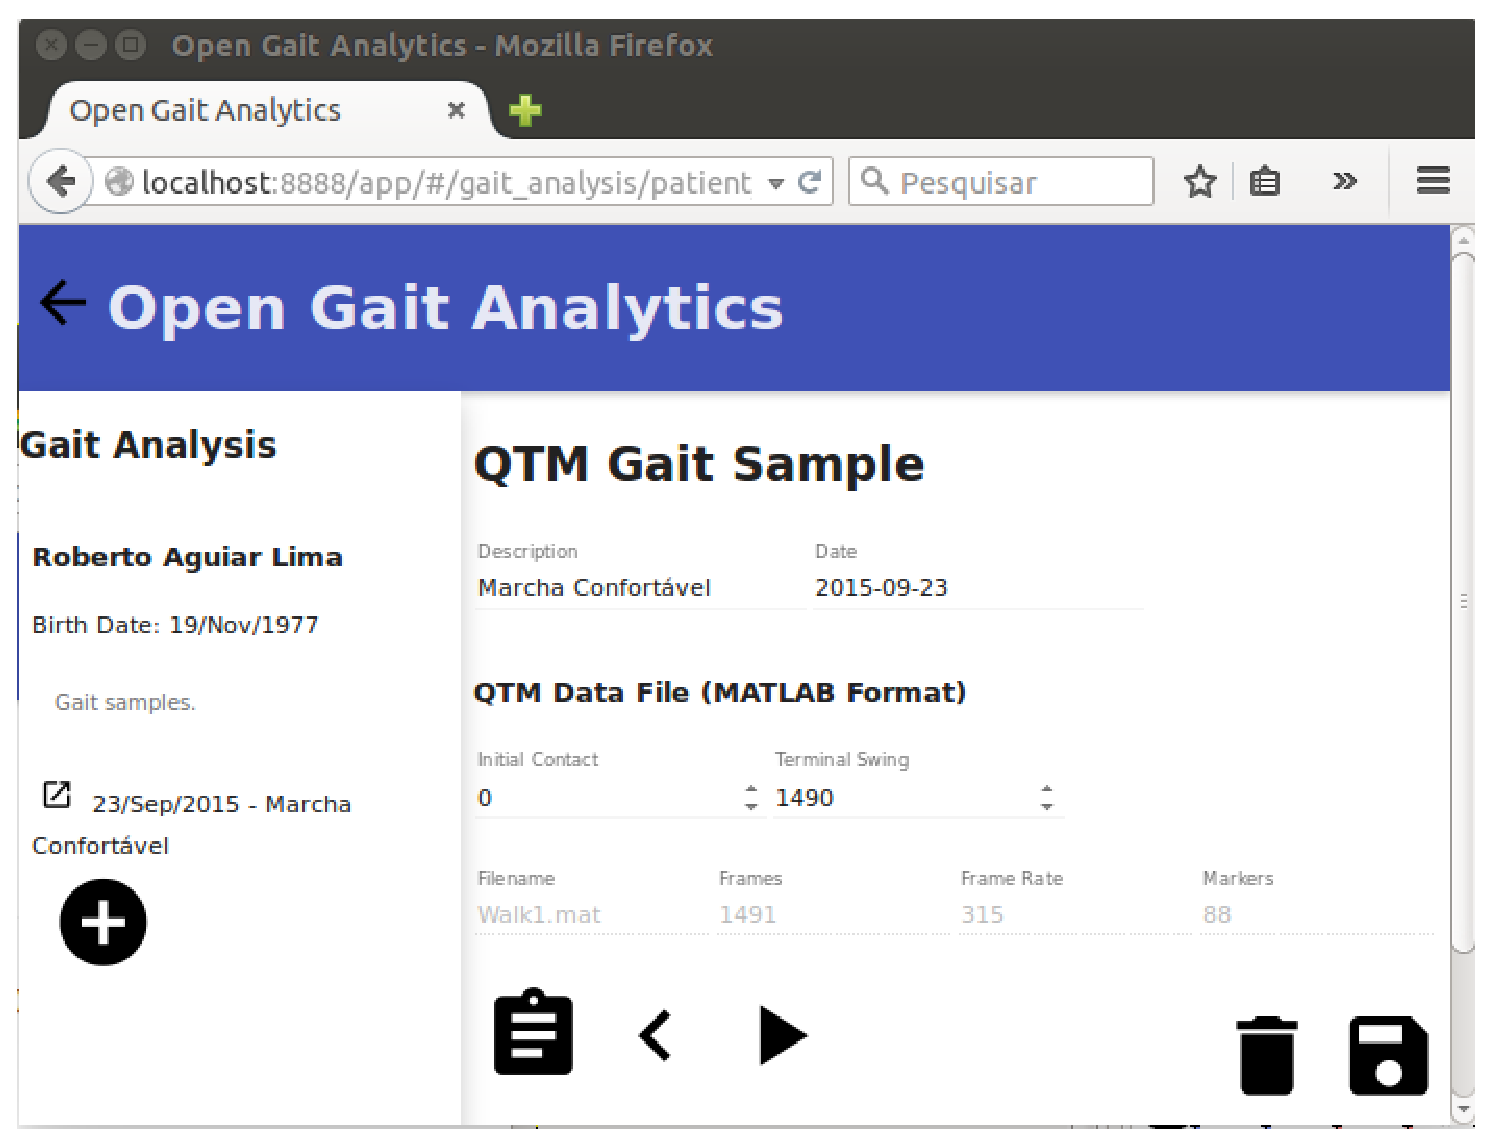
\includegraphics[width=\textwidth]{tela7}}
	\caption{Dados importados do QTM. }
	\label{qtm_data}
\end{figure*}


A partir desta tela é possível executar uma animação dos dados coletados (Fig. \ref{animacao}).
Nesta tela é possífel acelerar ou desacelerar, aplicar zoom in e zoom out, fazer pan e visualizar
um quadro específico da animação. O recurso de visualizar o quadro é importante pois é com ele
que se deve descobrir o quadro referente ao contato inicial e ao balanço terminal. Estes
dados devem ser cadastrados na tela mostrada na Fig. \ref{qtm_data}. Sem este procedimento não
é possível visualisar os gráficos de progreção espacial e de ângulos.

\begin{figure*}[tb]
	\centering
	{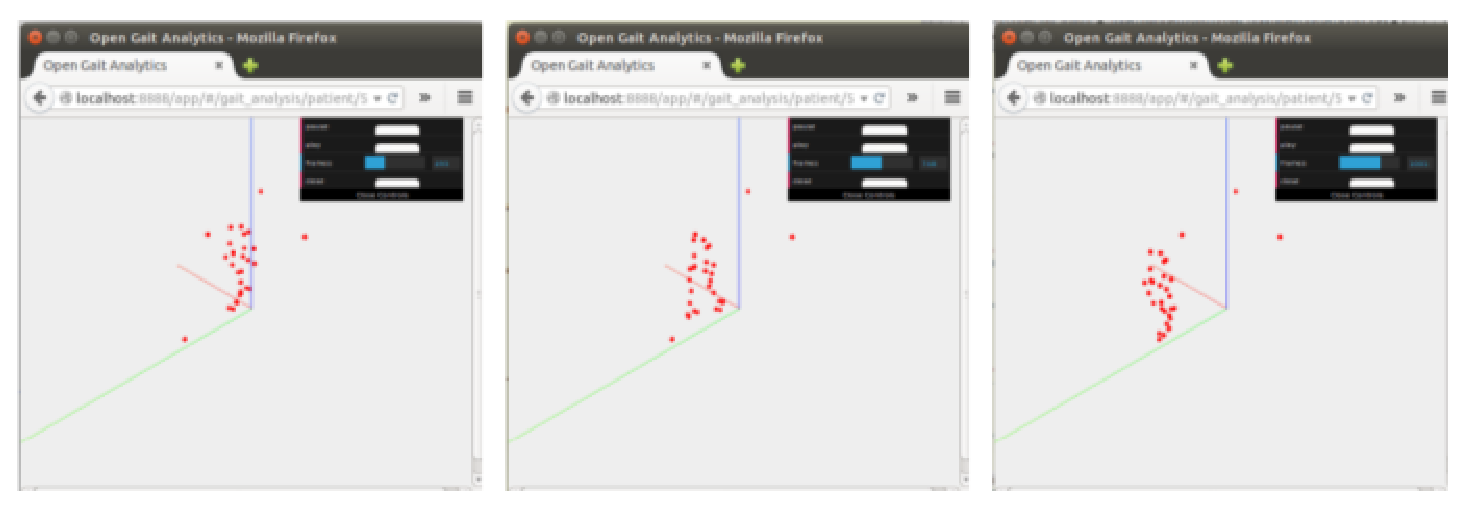
\includegraphics[width=\textwidth]{animacao}}
	\caption{Animação em 3D dos dados coletados. A) Contato inicial
		do membro inferior esquerdo. B) Membro inferior esquerdo no
	período de balanço. C) Membro inferior esquerdo no balanço terminal. }
	\label{animacao}
\end{figure*}

O software permite a nomeação dos marcadores vistos na animação. Depois de se nomear um marcador
específico, por exemplo, o calcâneo esquerdo, é possível ver sua progressão espacial como na 
Fig. \ref{progressao}.

\begin{figure}[!t]
	\centering
	{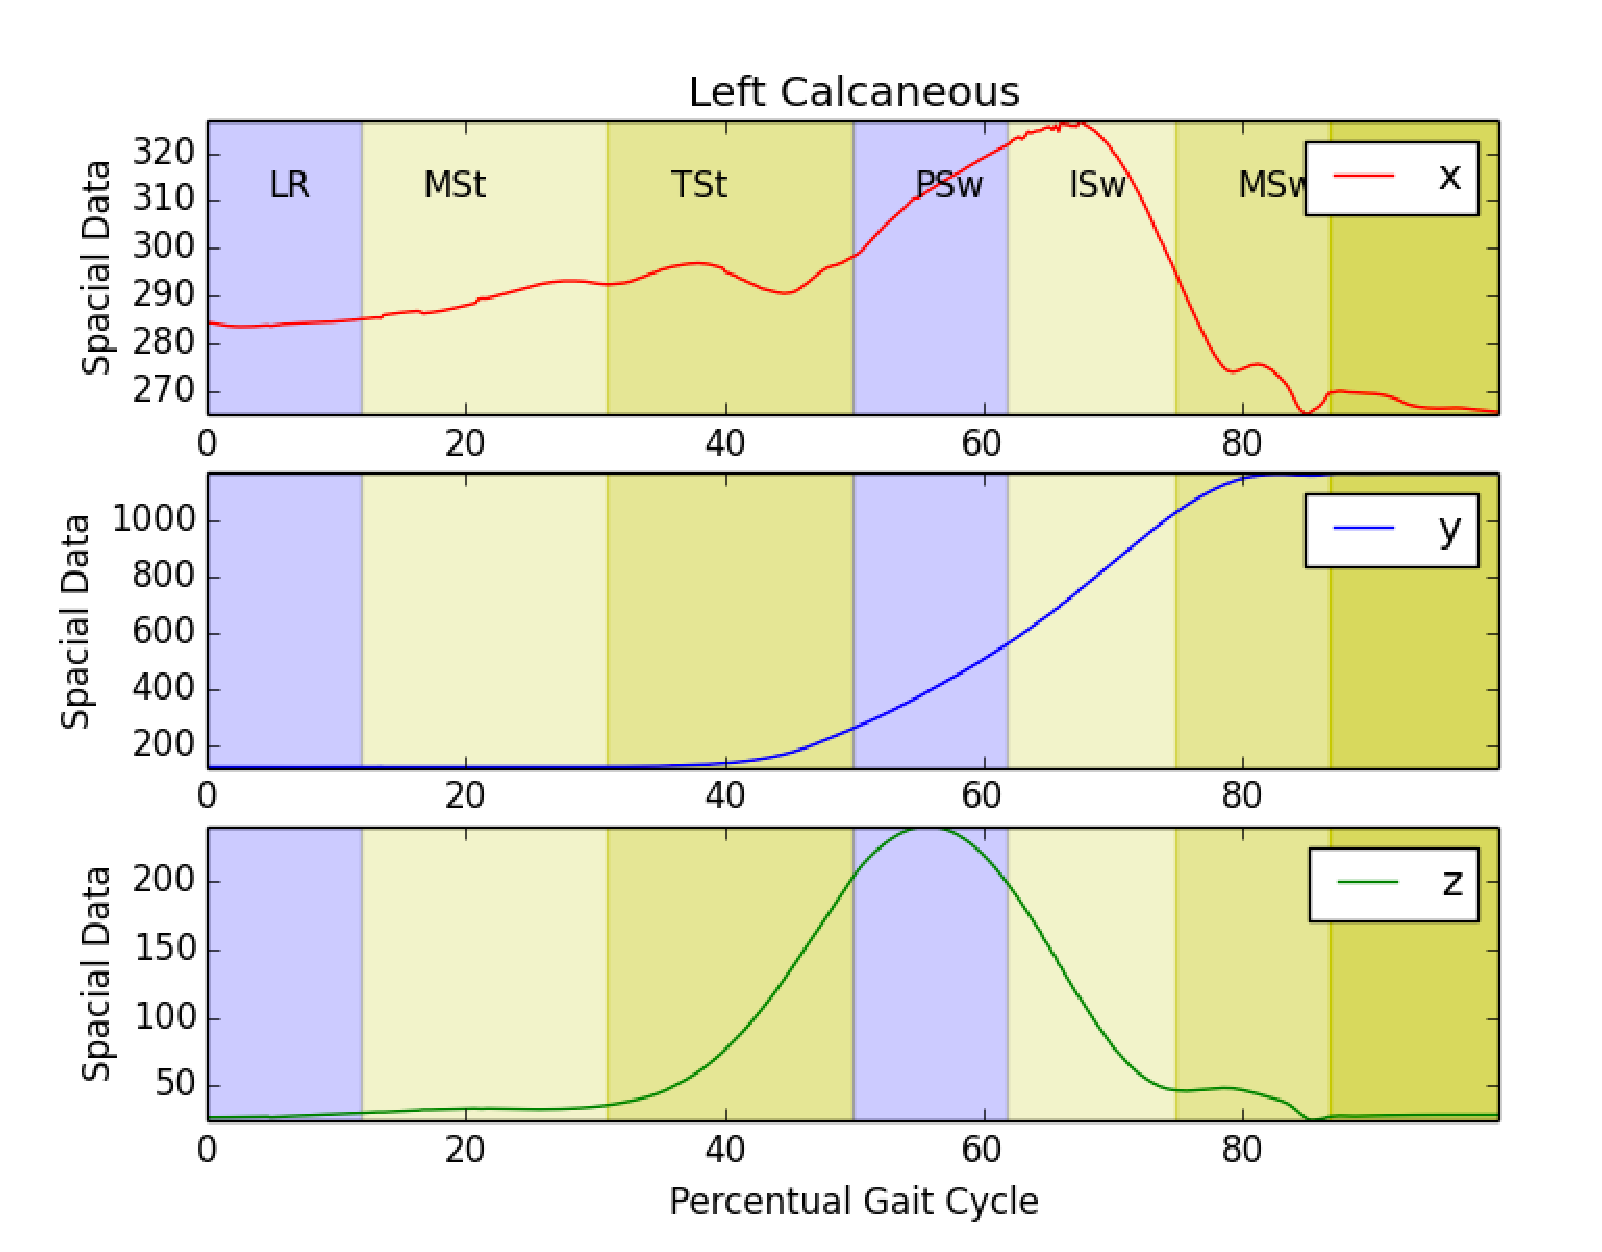
\includegraphics[width=9cm]{tela19}}
	\caption{Progressão no espaço do calcâneo esquerdo. }
	\label{progressao}
\end{figure}

Outro recurso importante da aplicação é o cadastramento de ângulos. 
Este recurso pode ser visto na Fig. \ref{angulos}. 
A partir desta tela é possível ver os ângulos (Fig. \ref{angulos}), velocidades angulares (Fig. \ref{va}) e
acelerações angulares (Fig. \ref{angular_accelerations}).

\begin{figure}[!t]
	\centering
	{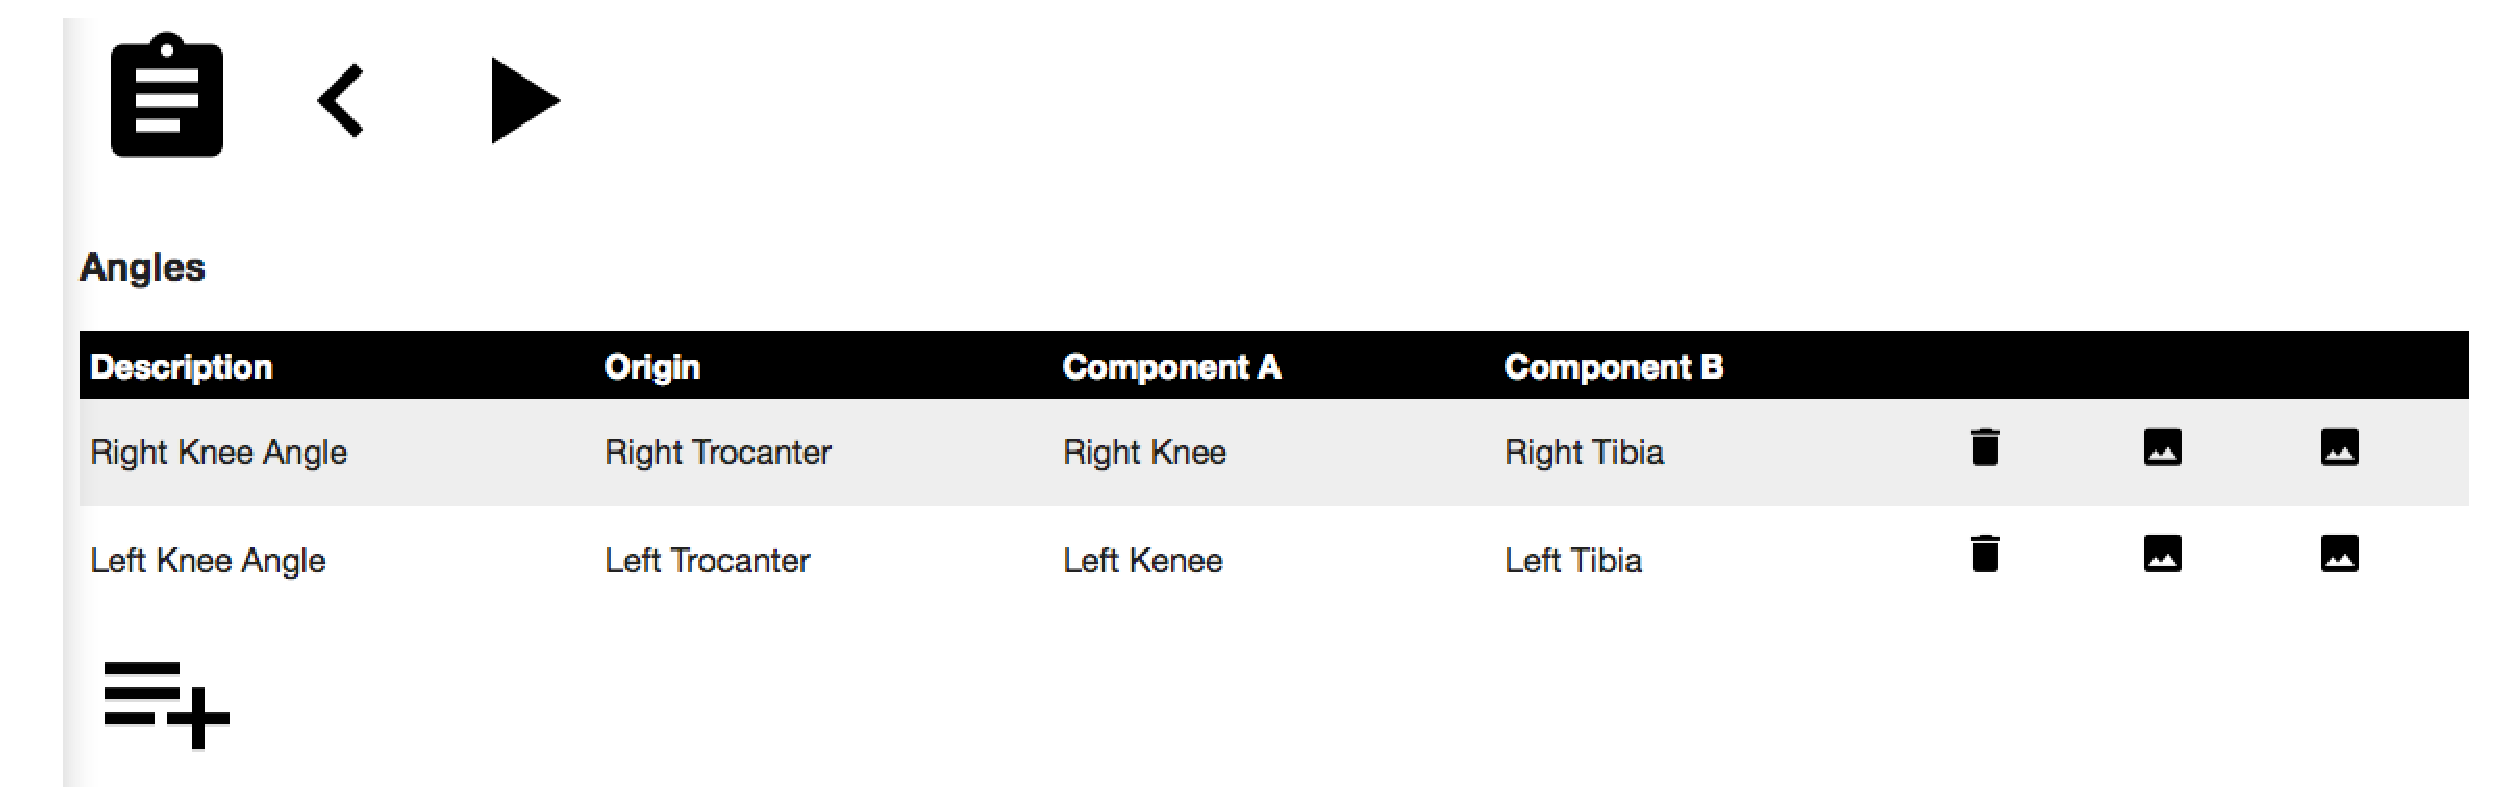
\includegraphics[width=9cm]{tela23}}
	\caption{Recurso para criação de ângulos. }
	\label{progressao}
\end{figure}

\begin{figure}[!t]
	\centering
	{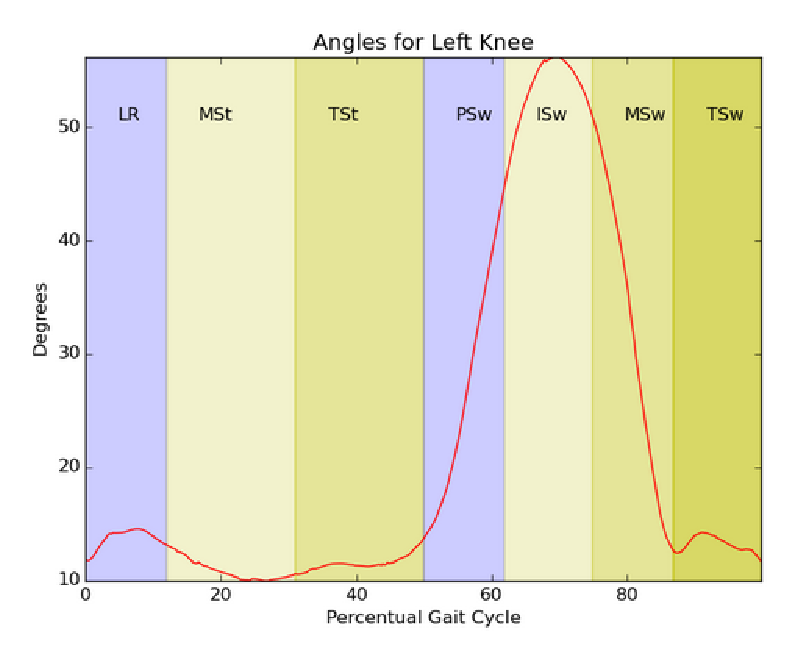
\includegraphics[width=9cm]{tela25}}
	\caption{Ângulo de um joelho. }
	\label{angulos}
\end{figure}

\begin{figure}[!t]
	\centering
	{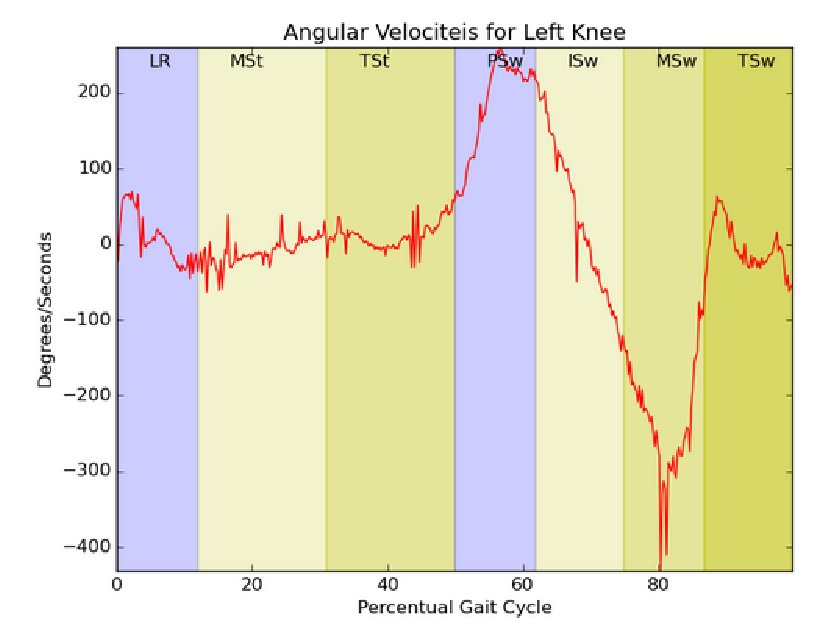
\includegraphics[width=9.5cm]{tela26}}
	\caption{Velocidades angulares de um joelho. }
	\label{va}
\end{figure}

\begin{figure}[!t]
	\centering
	{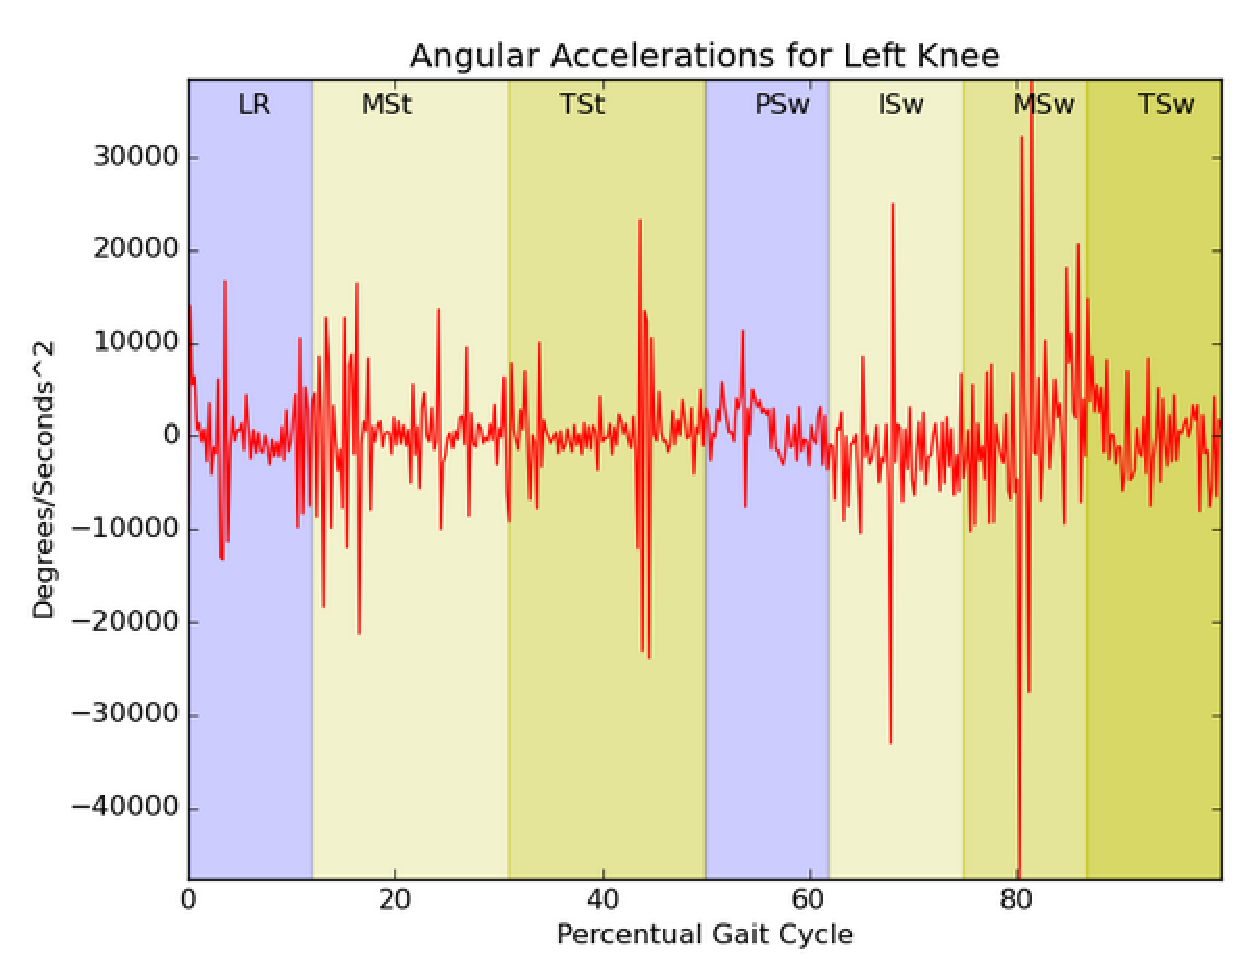
\includegraphics[width=9.5cm]{angular_accelerations}}
	\caption{Acelerações angulares de um joelho.}
	\label{angular_accelerations}
\end{figure}

\section{Discussão}

A criação de um software específico para análise de marcha totalmente disponível em ambiente web é
uma inovação na área. A maior vantagem deste enfoque é a fácil disponibilização do software,
que depois de ter uma versão implantada na internet, pode ser acessado de qualquer parte do mundo,
desde que o usuário tenha acesso a um browser HTM5 recente.
Outro tema importante a ser levantado sobre este projeto, é a possibilidade de se formar uma base
com dados de marcha humana coletados ao redor do globo, isso por si só seria de valor inestimável
a pesquisadores da área.

O software está disponibilizado como software livre. A intenção da equipe é atrair outros desenvolvedores
e profissionais de saúde que contribuam e usufruam do mesmo. Também não se descarta a idéia de se
criar um projeto para crowdfounding e assim permitir que mais pessoas contribuam com o mesmo, além
é claro de se conseguir recurso para mantê-lo.

Como trabalhos futuros, espera-se que novos métodos de coletas de dados sejam suportados, como por exemplo, plataformas de forças, EMG e IMU. Além disso, um módulo de simulações está sendo desenvolvido e se espera 
anexar métodos de aprendizado de máquina para classificação e regressão.


% needed in second column of first page if using \IEEEpubid
%\IEEEpubidadjcol

% An example of a floating figure using the graphicx package.  % Note that \label must occur AFTER (or within) \caption.  % For figures, \caption should occur after the \includegraphics.
% Note that IEEEtran v1.7 and later has special internal code that
% is designed to preserve the operation of \label within \caption
% even when the captionsoff option is in effect. However, because
% of issues like this, it may be the safest practice to put all your
% \label just after \caption rather than within \caption{}.
%
% Reminder: the "draftcls" or "draftclsnofoot", not "draft", class
% option should be used if it is desired that the figures are to be
% displayed while in draft mode.
%
%\begin{figure}[!t]
%\centering
%\includegraphics[width=2.5in]{myfigure}
% where an .eps filename suffix will be assumed under latex, 
% and a .pdf suffix will be assumed for pdflatex; or what has been declared
% via \DeclareGraphicsExtensions.
%\caption{Simulation results for the network.}
%\label{fig_sim}
%\end{figure}

% Note that IEEE typically puts floats only at the top, even when this
% results in a large percentage of a column being occupied by floats.


% An example of a double column floating figure using two subfigures.
% (The subfig.sty package must be loaded for this to work.)
% The subfigure \label commands are set within each subfloat command,
% and the \label for the overall figure must come after \caption.
% \hfil is used as a separator to get equal spacing.
% Watch out that the combined width of all the subfigures on a 
% line do not exceed the text width or a line break will occur.
%
%\begin{figure*}[!t]
%\centering
%\subfloat[Case I]{\includegraphics[width=2.5in]{box}%
%\label{fig_first_case}}
%\hfil
%\subfloat[Case II]{\includegraphics[width=2.5in]{box}%
%\label{fig_second_case}}
%\caption{Simulation results for the network.}
%\label{fig_sim}
%\end{figure*}
%
% Note that often IEEE papers with subfigures do not employ subfigure
% captions (using the optional argument to \subfloat[]), but instead will
% reference/describe all of them (a), (b), etc., within the main caption.
% Be aware that for subfig.sty to generate the (a), (b), etc., subfigure
% labels, the optional argument to \subfloat must be present. If a
% subcaption is not desired, just leave its contents blank,
% e.g., \subfloat[].


% An example of a floating table. Note that, for IEEE style tables, the
% \caption command should come BEFORE the table and, given that table
% captions serve much like titles, are usually capitalized except for words
% such as a, an, and, as, at, but, by, for, in, nor, of, on, or, the, to
% and up, which are usually not capitalized unless they are the first or
% last word of the caption. Table text will default to \footnotesize as
% IEEE normally uses this smaller font for tables.
% The \label must come after \caption as always.
%
%\begin{table}[!t]
%% increase table row spacing, adjust to taste
%\renewcommand{\arraystretch}{1.3}
% if using array.sty, it might be a good idea to tweak the value of
% \extrarowheight as needed to properly center the text within the cells
%\caption{An Example of a Table}
%\label{table_example}
%\centering
%% Some packages, such as MDW tools, offer better commands for making tables
%% than the plain LaTeX2e tabular which is used here.
%\begin{tabular}{|c||c|}
%\hline
%One & Two\\
%\hline
%Three & Four\\
%\hline
%\end{tabular}
%\end{table}


% Note that the IEEE does not put floats in the very first column
% - or typically anywhere on the first page for that matter. Also,
% in-text middle ("here") positioning is typically not used, but it
% is allowed and encouraged for Computer Society conferences (but
% not Computer Society journals). Most IEEE journals/conferences use
% top floats exclusively. 
% Note that, LaTeX2e, unlike IEEE journals/conferences, places
% footnotes above bottom floats. This can be corrected via the
% \fnbelowfloat command of the stfloats package.



\section{Conclusion}
O presente trabalho apresentou o software desenvolvido pelo LIS FGA/UnB em cooperação com o o LPH FCE/UnB.
O código fonte do projeto foi disponibilizado sob a licença MIT \cite{MIT2015} no endereço web http://github.com/rob-nn/open\_gait\_analytics.

O software conta com recursos para importação de dados oriundos do software QTM da Qualisys.
Permite fazer a nomeação de marcadores fixados no corpo do paciente no momento da coleta, 
além de habilitar a visualisação destes dados em gráficos. Também é possível cadastrar ângulos
e visualizá-los em gráficos assim como suas velocidades angulares.
Uma animação em 3D com os dados é visualizável. Todos os gráficos são visualizados de acordo com 
as fase do ciclo de marcha.

O sistema é implantável na internet e é acessível através de um browser HTML5 recente.
Ele também terá sua continuidade, implantação e adição de novos recursos, sob a tutela do LIS FGA/UnB e 
do LPH FCE/UnB.





% if have a single appendix:
%\appendix[Proof of the Zonklar Equations]
% or
%\appendix  % for no appendix heading
% do not use \section anymore after \appendix, only \section*
% is possibly needed

% use appendices with more than one appendix
% then use \section to start each appendix
% you must declare a \section before using any
% \subsection or using \label (\appendices by itself
% starts a section numbered zero.)
%


%\appendices
%\section{Proof of the First Zonklar Equation}
%Appendix one text goes here.

% you can choose not to have a title for an appendix
% if you want by leaving the argument blank
%\section{}
%Appendix two text goes here.


% use section* for acknowledgment
\section*{Acknowledgment}

O primeiro autor agradece ao apoio financeiro concedido pela Coordenação de Aperfeiçoamento de Pessoal de Nível Superior (CAPES) para realização do projeto.
Os autores agradecem também ao LIS FGA/UnB e ao LPH FCE/UnB, pela disponibilização de equipamentos e instalações para a execução do projeto.




% Can use something like this to put references on a page
% by themselves when using endfloat and the captionsoff option.
\ifCLASSOPTIONcaptionsoff
  \newpage
\fi



% trigger a \newpage just before the given reference
% number - used to balance the columns on the last page
% adjust value as needed - may need to be readjusted if
% the document is modified later
%\IEEEtriggeratref{8}
% The "triggered" command can be changed if desired:
%\IEEEtriggercmd{\enlargethispage{-5in}}

% references section

% can use a bibliography generated by BibTeX as a .bbl file
% BibTeX documentation can be easily obtained at:
% http://www.ctan.org/tex-archive/biblio/bibtex/contrib/doc/
% The IEEEtran BibTeX style support page is at:
% http://www.michaelshell.org/tex/ieeetran/bibtex/
\bibliographystyle{IEEEtran}
% argument is your BibTeX string definitions and bibliography database(s)
\bibliography{IEEEabrv,./IEEE.bib}
%
% <OR> manually copy in the resultant .bbl file
% set second argument of \begin to the number of references
% (used to reserve space for the reference number labels box)


% biography section
% 
% If you have an EPS/PDF photo (graphicx package needed) extra braces are
% needed around the contents of the optional argument to biography to prevent
% the LaTeX parser from getting confused when it sees the complicated
% \includegraphics command within an optional argument. (You could create
% your own custom macro containing the \includegraphics command to make things
% simpler here.)
%\begin{IEEEbiography}[{\includegraphics[width=1in,height=1.25in,clip,keepaspectratio]{mshell}}]{Michael Shell}
% or if you just want to reserve a space for a photo:

\begin{IEEEbiography}[{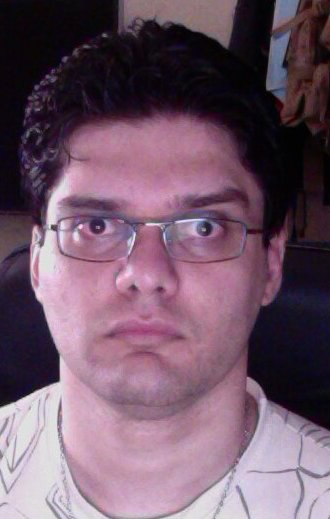
\includegraphics[width=1in,height=1.25in,clip,keepaspectratio]{roberto}}]{Roberto Aguiar Lima}
	Possui graduação na área em Ciência da Computação pela Universidade Católica de Brasília (2000).
	Atualmente cursa o programa de Mestrado em Engenharia Biomédica da Universidade de Brasília.
	Possui mais de 20 anos como desenvolvedor de software.
\end{IEEEbiography}

% if you will not have a photo at all:
\begin{IEEEbiography}[{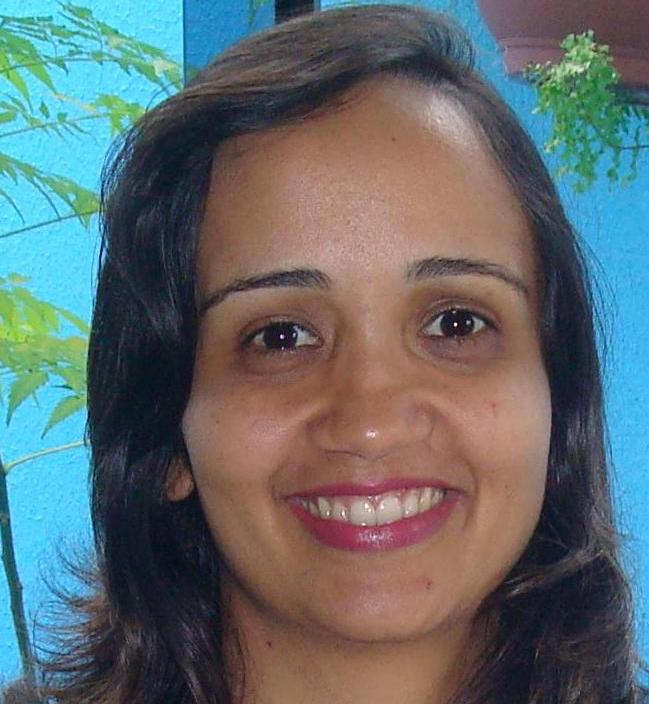
\includegraphics[width=1in,height=1.25in,clip,keepaspectratio]{vera}}]{Vera Regina Da Silva Marães}
Possui graduação em Fsioterapia pela Universidade Federal de São Carlos (1995), mestrado em Biologia Celular e Estrutural pela Universidade Estadual de Campinas (1999) e doutorado em Fisioterapia pela Universidade Federal de São Carlos (2004). Atualmente é docente adjunto III da Faculdade de Ceilândia; do Programa de Pós-Graduação em Engenharia Biomédica e do Pro-Ensino na Saúde da Universidade de Brasília. Tem experiência na área de Fisioterapia, atuando principalmente nos seguintes temas: ensino na saúde, adaptação de próteses em amputados, funcionalidade humana, fisiologia do exercício, reabilitação cardíaca e variabilidade da frequência cardíaca.
\end{IEEEbiography}

% insert where needed to balance the two columns on the last page with
% biographies
%\newpage

\begin{IEEEbiography}[{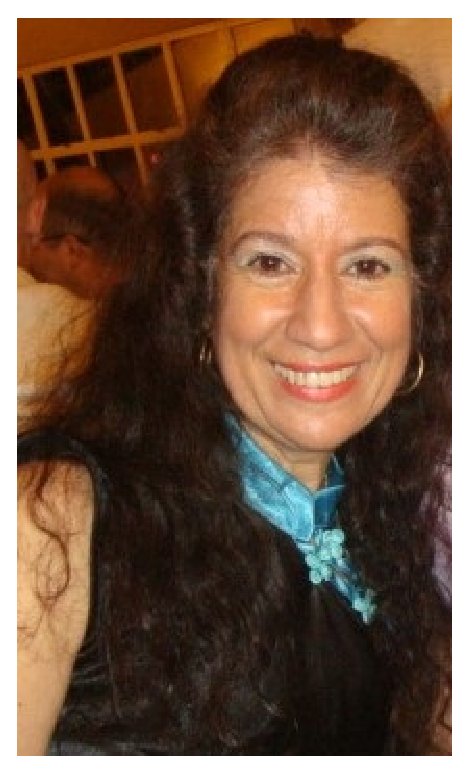
\includegraphics[width=1in,height=1.25in,clip,keepaspectratio]{lourdes}}]{Lourdes Mattos Brasil}
Lourdes Mattos Brasil possui graduação em Engenharia Elétrica pela Universidade Federal de Santa Catarina (1989), 
Mestrado em Engenharia Elétrica/Engenharia Biomédica pela Universidade Federal de Santa Catarina (1994) e 
concluiu o doutorado em Engenharia Elétrica/Sistemas de Informação - Engenharia Biomédica pela Universidade Federal de Santa Catarina em 1999, 
sendo parte realizado na Facultés Universitaires Notre-Dame de La Paix (FUNDP), Namur  Belgium (1998). 
Realizou estágio Pós-Doutoral no Programa de Pós-Graduação em Engenharia Biomédica da Universidade Federal da Paraíba (2001-2002). 
Atualmente é Professor Adjunto da Universidade de Brasília (UnB), 
Faculdade UnB-Gama (FGA), onde atua na Engenharia Eletrônica, 
bem como é coordenadora do Lato Sensu em Engenharia Clínica e dos Laboratórios de Informática em Saúde (LIS) e de Nanotecnologia (NTEC-FGA). 
Também é pesquisadora/docente do Stricto Sensu, Mestrado em Engenharia Biomédica. 
Tem experiência na área de Engenharia Biomédica, com ênfase em Informática em Saúde, atuando principalmente nos seguintes temas: 
informática em saúde, inteligência artificial em saúde, engenharia biomédica, redes neurais artificiais, sistemas baseados no conhecimento, descoberta de conhecimento, realidade virtual, sistemas tutores inteligentes, sistemas especialistas híbridos, sistemas inteligentes, processamento de imagens, nanotecnologia e gestão do conhecimento. 
Suas produções técnicas-científicas permeiam essas áreas, bem como suas publicações de livros, prêmios, palestras/seminários, pareceres, consultorias. 
Também participa como membro das sociedades brasileira e internacional: SBC, SBEB e IEEE.
\end{IEEEbiography}

% You can push biographies down or up by placing
% a \vfill before or after them. The appropriate
% use of \vfill depends on what kind of text is
% on the last page and whether or not the columns
% are being equalized.

%\vfill

% Can be used to pull up biographies so that the bottom of the last one
% is flush with the other column.
%\enlargethispage{-5in}



% that's all folks
\end{document}


